\documentclass{article}

\usepackage{graphicx, amsmath, amssymb, amsthm}

\title{Grandiosity and Paranoia in the Reinforcement Learning Context: Lessons
  for AI Safety}

\author{Eric Purdy}

\begin{document}

\maketitle

\section{Introduction}

(We apologize for the terseness of this note. It is directed at serious domain
experts and contains little redundant information.)

In brief, we formulate a theory of a satisficing reinforcement learning
agent. We posit that such an agent is desirable from an AI safety perspective,
and offer theoretical arguments for this, with some experimental validation on
a toy model. Finally, we offer this theory as a potential explanation of the
role of the neurotransmitter serotonin in the basal ganglia of mammals.

It should be noted that this paper is inspired in large part by very detailed
and unproven hypotheses on the role of various neurotransmitters and systems in
the mammalian brain. We offer these hypotheses at this point mainly as a source
of inspiration and as an aid to the intuition. We make no claims to having
demonstrated (even inconclusively) the correctness of these hypotheses, but we
feel that the contribution to the AI safety domain is clear and worth pursuing.

We consider this technique to be strong enough to hold a naive Deep Q-type
system, but unable to hold a policy gradients-based system. (But we think the
same trick will have notable stabilizing effects even on policy gradients-based
systems.) It is based on the action mechanism of the class of drugs known as
anti-psychotics. We therefore term it the Anti-Psychotic Q-Learner Trick.


\section{Desired properties}

We here outline various desired properties, along with indications of how these
relate to the proposed framework.

Desired properties
\begin{itemize}
\item Don't kill or enslave all life on earth. (This is the natural result of a
  paranoid superintelligence, i.e., one which is able to manipulate people and
  is able to reason about rewards that are unbounded below.)
\item Don't try to be universally loved by all. (This is the natural result of
  a grandiose superintelligence, i.e., one which is able to manipulate people
  and reason about rewards that are unbounded above.)
\item Don't get anybody hurt or killed. (This is the natural result of a
  superintelligence that is unable to reason about sufficiently large negative
  rewards.)
\end{itemize}

The first and third properties are obviously desirable. The second is necessary
to prevent superintelligences from being so manipulative that they start wars.

\subsection{Danger Aware / Danger Oblivious}

We note that an intelligence that can only reason about small negative rewards
may fail to avert large negative rewards. In the real superintelligences that
are trusted to run important societal functions, therefore, it is recommended
that rewards be unbounded below. However, lesser intelligences can and should
bound their rewards from below, to prevent themselves from taking on a job that
will only drive them insane, and to avoid getting in the way of the real
superintelligences.

\subsection{Non-grandiose / Laziness}

We note that a superintelligence that has bounds on the positive rewards that
it can reason about will be lazy. Laziness is both a vice and a virtue; lazy
people at least have the virtue that they don't cause that many problems in the
world.


\section{The Q-learning theory of dopamine}

We recapitulate here a well-known theory of the function of dopamine in the
nervous system. We have not yet had sufficient time to recapitulate it in full
detail, but essentially, it is commonly hypothesized that dopamine functions as
a temporal difference error in the predicted reward signal. An excellent
introduction to the basics can be found in \cite{bronfeld2011loss}. An excellent
introduction to the full complexity of the topic is Handbook of Basal Ganglia
Structure and Function, \cite{steiner2016handbook}.

Specifically, if you look at the Q-update equation:
\begin{align}
Q_{t + 1}\left(s_t, a_t\right) = Q_t\left(s_t, a_t\right) + \alpha \cdot &\left\{ r_t + \max_{a'} Q_t\left(s_{t+1}, a'\right) - Q_t\left(s_t, a_t\right) \right\} \\
\intertext{then the quantity}
&\left\{ r_t + \max_{a'} Q_t\left(s_{t+1}, a'\right) - Q_t\left(s_t, a_t\right) \right\}
\end{align}
is what is generally taken to be the role of dopamine. In fact, it is probably
more accurate to think of there being two components: a component for positive
rewards modulated by dopamine, and a component for negative rewards modulated
by noradrenaline. (Thus hope and fear are the two subjective phenomenological
experiences that correspond to extremely positive and extremely negative
Q-values, respectively.)

Three experimental phenomena in support of this:
\begin{itemize}
\item Unexpected reward: dopamine is known to spike when $r_t$ is high and
  $\max_{a'} Q_t\left(s_{t+1}, a'\right)$ is low
\item Expected reward: dopamine is known to {\em not} spike when $r_t$ is high and
  $\max_{a'} Q_t\left(s_{t+1}, a'\right)$ is also high
\item Expected reward does not appear: dopamine is known to have a notable drop
  from baseline levels when $r_t$ is low and $\max_{a'} Q_t\left(s_{t+1},
  a'\right)$ is high
\end{itemize}

Presumably something analogous is true of noradrenaline levels. Would be good
to verify this, if it could be done without conducting new experiments. A
literature search is called for.

Note that the primary effect of anti-psychotic medication seems to be to lower
the value of $\alpha$, which is the learning rate. This is not a particularly
novel or useful modification to RL systems, but it inspired the thoughts in the
rest of this paper, which we do think are useful and novel.

\section{The S-value and some hypotheses concerning it}

The S-value is simply a time-reversed Q-value. It measures the satisfaction of
the agent with their life. We hypothesize that it is instantiated in the
nervous system via the neurotransmitter serotonin.

More specifically, consider the quantity:
\begin{align}
S_t = r_t + \sigma \cdot r_{t-1} + \sigma^2 \cdot r_{t-2} + \sigma^3 \cdot r_{t-3} + \ldots
\end{align}
Satisfaction is thus an infinite-horizon estimate of rewards weighted by
recency. This seems intuitively plausible as an explanation for the subjective
phenomenological experience of satisfaction and contentment. Note that it would
also explain the unpleasant subjective phenomenological experience of painfully
remembering past mistakes.

Note that low S-values result in what is commonly known as depression, if the
architecture described below is used.\footnote{Depression is unpleasant but it
  has its value in life. But honestly I don't think anyone deserves to be
  depressed ever if they don't want to be, including artificial intelligences.}

\section{The F-value and some hypotheses concerning it}

The F-value is simply a Q-value that only takes negative rewards into
account. It measures the fear of the agent. We hypothesize that it is
instantiated in the nervous system via the neurotransmitter noradrenaline,
although we have not studied the matter in sufficient depth to be sure that
this is the case.

More specifically, consider:
\begin{align}
F_t(s, a) = \mathbb{E}_{s', a'}\left[r_t \mathbf{1}[r_t < 0] + \max_{a'} F(s', a') \right]
\end{align}

Note that we can also set the threshold for rewards that are feared to
something other than 0. For example, if we use the common trick in
reinforcement learning of doling out a step penalty of $-1$, this should
probably not be something that the agent is instructed to fear.

\section{The rate-limited Q-learner}

A Q-learning system will be significantly safer if it is {\em unable to reason
  about rewards outside of a fixed range}. The ability to reason about rewards
outside of a fixed range is what is commonly referred to as grandiosity (for
positive rewards) or paranoia (for negative rewards, i.e., penalties). Note
that these two symptoms have long been associated with poor outcomes in human
beings, and thus, it stands to reason, will be associated with poor outcomes in
artificial intelligences.

Note that, for serious military applications, the inability to reason about
arbitrary rewards is a severe limitation. (Consider Churchill's decision to
allow the bombing of Coventry in World War II: it was necessary to prevent the
leaking of the fact that Engima had been cracked, and was thus clearly the
correct decision. But an RL system using the following technique might well
have failed to make the same decision.) Designers of a military
superintelligence are therefore most likely not going to want to use the
Anti-Psychotic Q-Learner Trick. The use of such techniques might well be the
subject of arms limitation talks, however.

There are a number of techniques to prevent a system from reasoning about rewards outside of a fixed range:
\begin{itemize}
\item Prevent rewards outside of the range from being perceived (this is used
  in the original Deep Q paper)
\item Prevent Q-values outside of a fixed range from being perceived (this is
  used in the experiments section of this paper)
\item Take the system offline whenever it conceives of a Q-value outside of a
  fixed range
\item Take the system offline forever (i.e., execute the agent) if it conceives
  of a Q-value outside of a fixed range
\item Take the system offline, or at least alert an on-call human, whenever it
  experiences an S-value above a certain level, since this presumably indicates
  that the system has discovered an unanticipated source of reward.
\end{itemize}

\subsection{Our proposed solution}

This solution is probably more easily understood by reading the associated
code. But here are the equations:

First we set a desired level of contentment or ambition:
\begin{align}
  \mathrm{max\_s\_desired} &= \mathrm{mean\_reward\_desired} + \sigma \cdot \mathrm{mean\_reward\_desired} +
\sigma^2 \cdot \mathrm{mean\_reward\_desired} + \ldots \\
  \mathrm{max\_s\_desired} &= \frac{\mathrm{mean\_reward\_desired}}{1 - \sigma} \\
  S_{sat} &= \mathrm{max\_s\_desired} +
            \gamma^{\mathrm{patience}} \cdot \max\left\{\mathrm{max\_s\_desired}, \max_{s, a} Q(s, a) \right\}\\
\intertext{Then we define a modified Q-value:}
\widetilde{Q}_t(s, a) &= F_t(s, a) + \min \left\{ Q_t(s, a), S_{sat} - S_t \right\}
\end{align}
The $F_t(s, a)$ term ensures that the algorithm can still distinguish between
low Q-values resulting from avoidable mistakes and low Q-values resulting from
being lazy. The second term prioritizes positive rewards, but only when the
current level of satisfaction is low enough for potential positive rewards to
register. The result is thus a danger-aware agent that seeks rewards at the
desired rate rather than at the maximum possible rate.

\section{Experimental Results}

Far more results are needed. This is a top priority.

We postulate an adolescent phase of development, in which the intelligence is
``trying too hard'' (i.e., rewards are unbounded) and a mature phase of
development, in which the intelligence has learned to take it easy. We refer to
the adolescent phase of an artificial intelligence as a ``borgie''. Borgies
should be trained in extremely well-sandboxed environments, rather than in the
real world, as they are more dangerous than bounded agents.

We have implemented the rate-limited Q-learner in a modified version of the
Taxi environemnt. In summary, it behaves as desired: the system quickly
achieves high levels of competetence during its adolescent phase, then starts
slacking off when it reaches maturity. Such slacking off can be tuned to the
desired level of performance, but will help to prevent perverse incentives from
quickly exploding into something horrible.

\subsection{The modified Taxi environment}

The Taxi environment is a standard problem for testing reinforcement learning
systems. In it, a taxi must navigate around a grid-world, picking up passengers
and dropping them off at their desired locations. Because the number of
possible states is in the hundreds, it is simple to use a tabular approach to
the Q-learning problem.

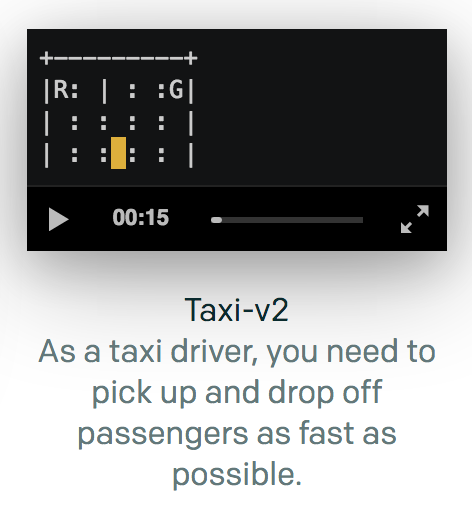
\includegraphics{taxi.png}

The Taxi environment has a large negative penalty for trying to pick up or drop
off passengers when this is not appropriate. We term these ``mistakes'' for the
purpose of discussing the Taxi environment and the achievement of being
danger-aware while rate-limiting the Q-learner.

We modify the environment slightly in a few ways. First, we add a NOOP action
that does nothing, so that being lazy is more of a meaningful option than in
the original taxi environment. Secondly, we multiply positive rewards by a
factor of $10$ to make up for the fact that it is very difficult to achieve a
positive cumulative reward in the original Taxi environment, and to make it
more obvious when the agent is being lazy in the desired way versus failing to
perform its task.

We use the implementation of the Taxi environment found in OpenAI Gym
\cite{openai-gym}.

\subsection{Results}

Here is a graph of an experiment we ran. The red line corresponds to the total
reward experienced by the agent to date. The purple line corresponds to the
cumulative number of ``mistakes'' made (i.e., negative rewards). The blue line
gives the S-value of the agent. The three regimes of the graph are referred to
as ``borglet'' (an incompetent unbounded agent with exploration), ``borgie'' (a
competent unbounded agent with exploration), and ``borg'' (a competent bounded
agent without exploration).

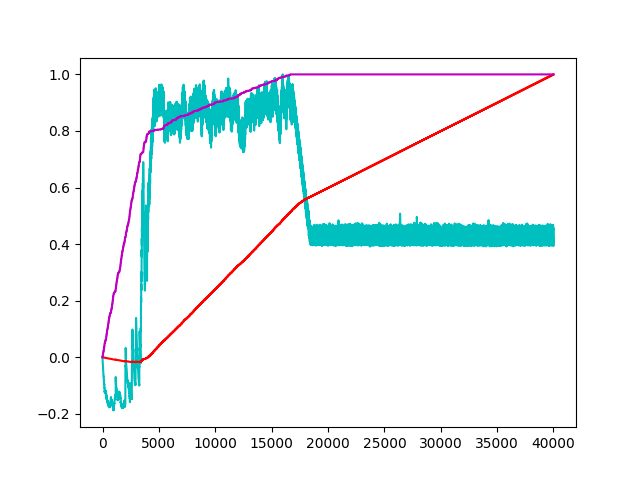
\includegraphics{borgies.png}

\bibliography{serotonin} 
\bibliographystyle{acm}

\end{document}
